%%%%%%%%%%%%%%%%%%%%%%%%%%%%%%%%%%%%%%%%%
% Jacobs Landscape Poster
% LaTeX Template
% Version 1.1 (14/06/14)
%
% Created by:
% Computational Physics and Biophysics Group, Jacobs University
% https://teamwork.jacobs-university.de:8443/confluence/display/CoPandBiG/LaTeX+Poster
% 
% Further modified by:
% Nathaniel Johnston (nathaniel@njohnston.ca)
%
% This template has been downloaded from:
% http://www.LaTeXTemplates.com
%
% License:
% CC BY-NC-SA 3.0 (http://creativecommons.org/licenses/by-nc-sa/3.0/)
%
%%%%%%%%%%%%%%%%%%%%%%%%%%%%%%%%%%%%%%%%%


\documentclass[final]{beamer}
\usepackage[scale=1.24]{beamerposter}
\usetheme{confposter}

%-----------------------------------------------------------
% Define the column widths and overall poster size
% To set effective sepwid, onecolwid and twocolwid values, first choose how many columns you want and how much separation you want between columns
% In this template, the separation width chosen is 0.024 of the paper width and a 4-column layout
% onecolwid should therefore be (1-(# of columns+1)*sepwid)/# of columns e.g. (1-(4+1)*0.024)/4 = 0.22
% Set twocolwid to be (2*onecolwid)+sepwid = 0.464
% Set threecolwid to be (3*onecolwid)+2*sepwid = 0.708

\newlength{\sepwid}
\newlength{\onecolwid}
\newlength{\twocolwid}
\newlength{\threecolwid}
\setlength{\paperwidth}{48in} % A0 width: 46.8in
\setlength{\paperheight}{36in} % A0 height: 33.1in
\setlength{\sepwid}{0.024\paperwidth} % Separation width (white space) between columns
\setlength{\onecolwid}{0.22\paperwidth} % Width of one column
\setlength{\twocolwid}{0.464\paperwidth} % Width of two columns
\setlength{\threecolwid}{0.708\paperwidth} % Width of three columns
\setlength{\topmargin}{-0.5in} % Reduce the top margin size
%-----------------------------------------------------------

\usepackage{graphicx}
\usepackage{booktabs}
\usepackage{multirow}
\title{Stimulus Identification from fMRI scans}

\author{Charles Zheng and Yuval Benjamini} % Author(s)

\institute{Stanford University, Department of Statistics} % Institution(s)

%----------------------------------------------------------------------------------------

\begin{document}

\addtobeamertemplate{block end}{}{\vspace*{2ex}} % White space under blocks
\addtobeamertemplate{block alerted end}{}{\vspace*{2ex}} % White space under highlighted (alert) blocks

\setlength{\belowcaptionskip}{2ex} % White space under figures
\setlength\belowdisplayshortskip{2ex} % White space under equations

\begin{frame}[t] % The whole poster is enclosed in one beamer frame

\begin{columns}[t] % The whole poster consists of three major columns, the second of which is split into two columns twice - the [t] option aligns each column's content to the top

\begin{column}{\sepwid}\end{column} % Empty spacer column

\begin{column}{\onecolwid} % The first column

%----------------------------------------------------------------------------------------
%	INTRODUCTION
%----------------------------------------------------------------------------------------

\setbeamercolor{block alerted title}{fg=white,bg=BlueViolet} % Change the alert block title colors
\setbeamercolor{block alerted body}{fg=black,bg=white} % Change the alert block body colors

\begin{alertblock}{Overview}
\vspace{0.3in}

Seeking to explain the processes behind human perception, scientists
employ \emph{forward models} to model the causal relationship between
perception of stimuli and neural activity.  But how can we measure the quality of
these models?  Kay et al (2008) introduced the
task of \emph{identification} as a way to demonstrate the fidelity and
generalizability of the model.
\vspace{0.6in}

Using the data of Kay \emph{et al.} as a motivating example, we
consider the statistical problem of optimal identification.  While
identification resembles a classification task (with
many classes), it combines the challenge of multivariate regression
with high-dimensional covariance estimation.
\end{alertblock}

\begin{block}{Data}
\begin{itemize}
\item Sequence of stimuli (pictures) shown at time $t = 1,\hdots, T = 3500$
\item Record subject's multivariate response $y_t \in \mathbb{R}^p$, here $p \approx 20000$ voxels
\end{itemize}

\begin{center}
\begin{tabular}{ccccc}
$t = 1$ & $t = 2$ & $t = 3$ & $t = 4$ & $\cdots$\\ \hline
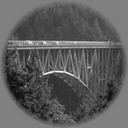
\includegraphics[scale = 0.8]{img1.png} &
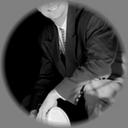
\includegraphics[scale = 0.8]{img2.png} &
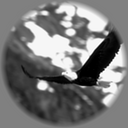
\includegraphics[scale = 0.8]{img3.png} &
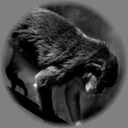
\includegraphics[scale = 0.8]{img4.png} & $\cdots$\\ \hline
$y_1$ & $y_2$ & $y_3$ & $y_4$ & $\cdots$\\ \hline
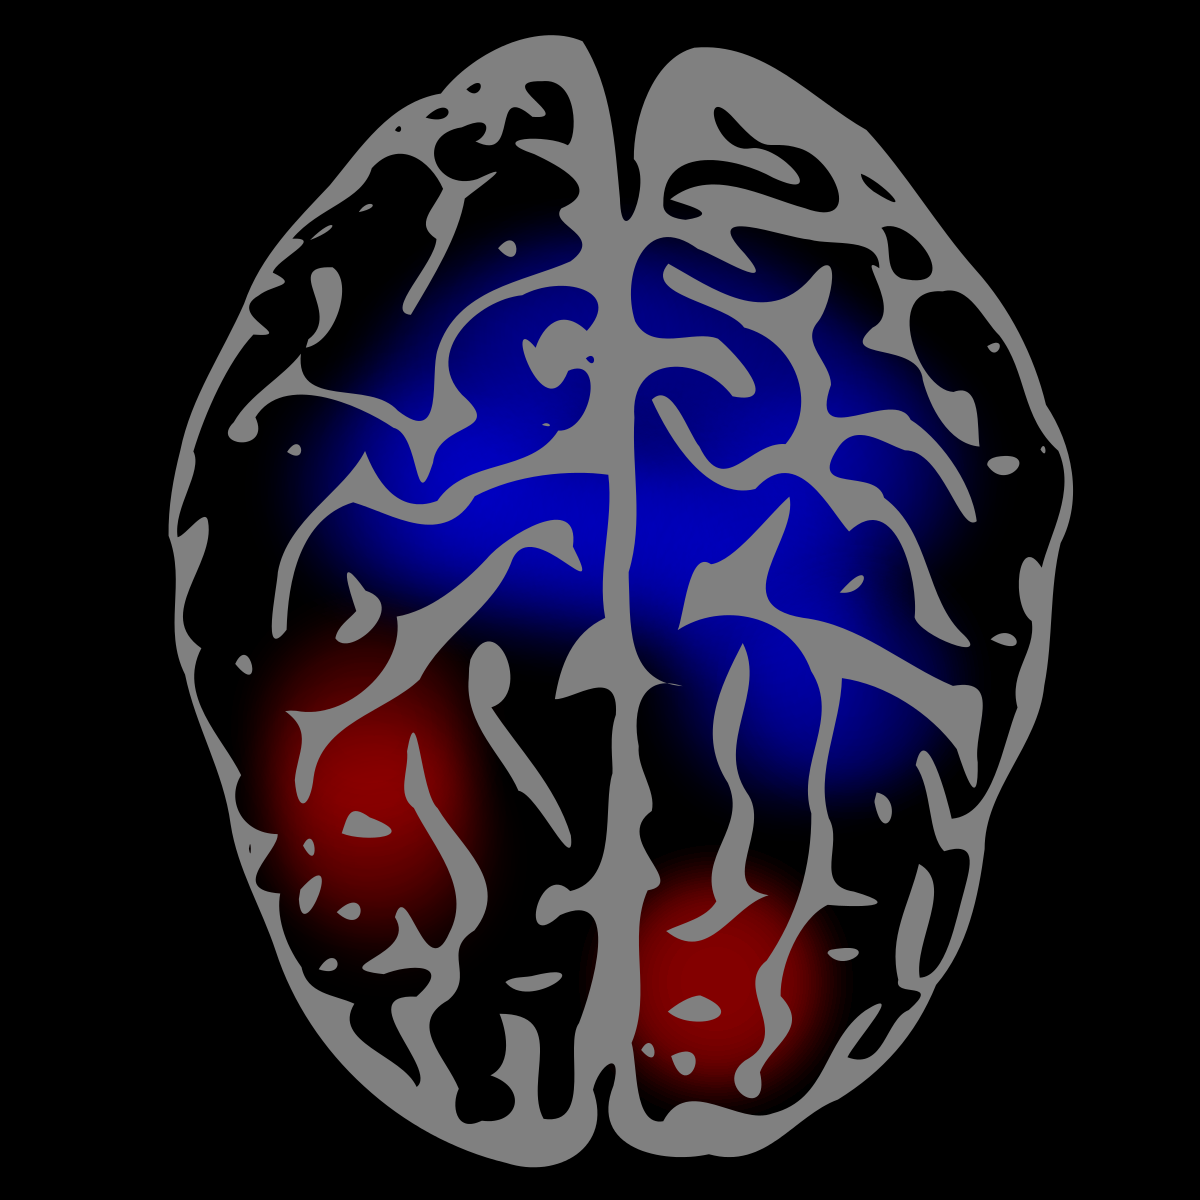
\includegraphics[scale = 0.10]{brain1.png} &
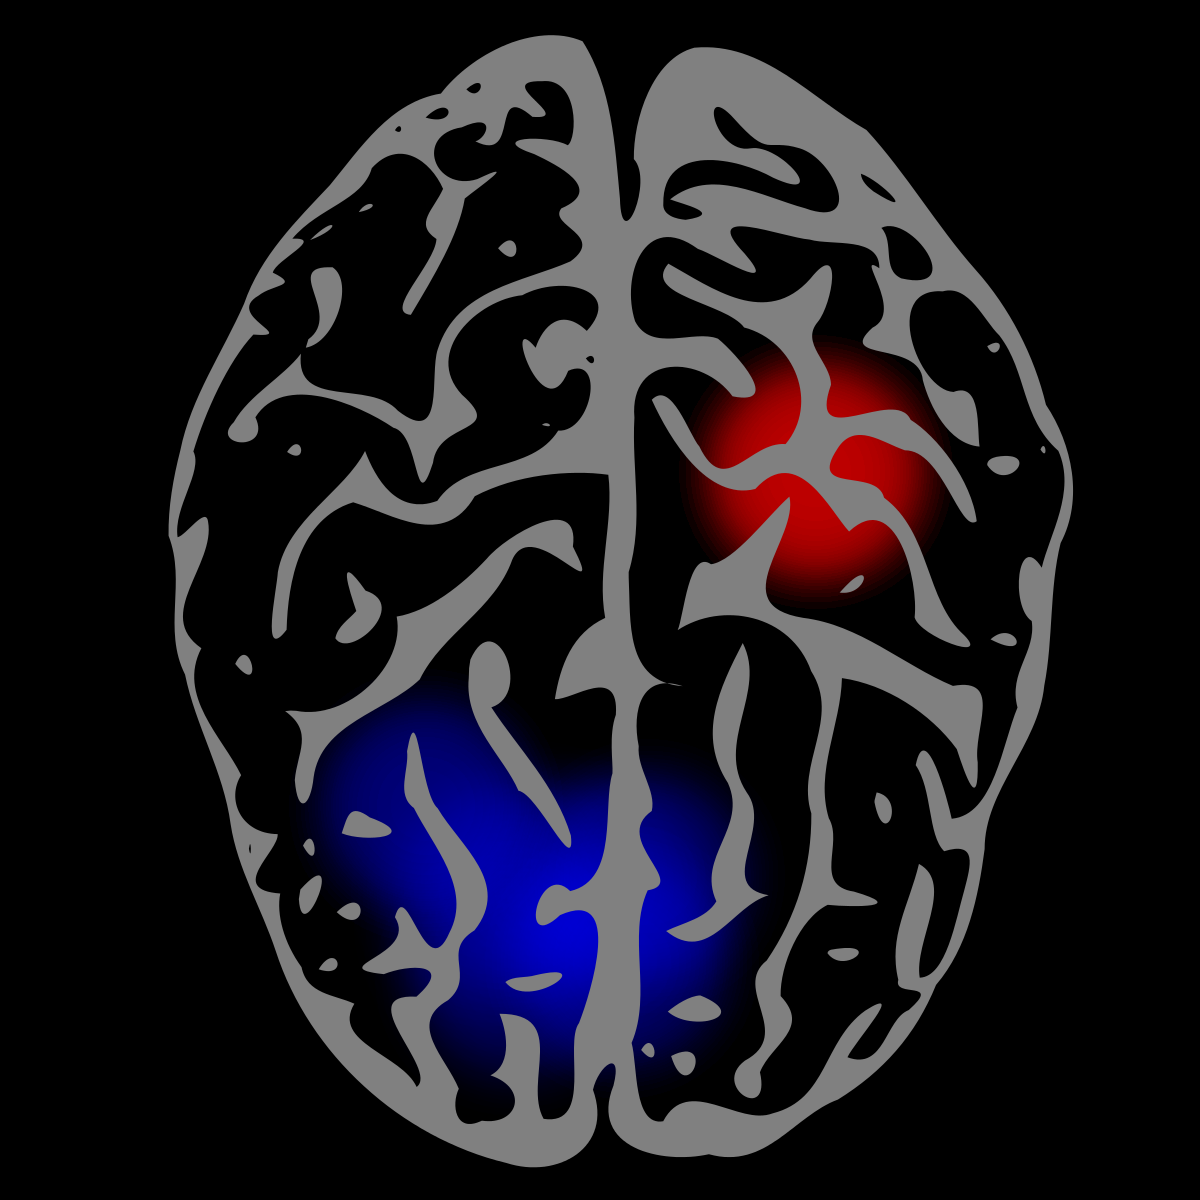
\includegraphics[scale = 0.10]{brain2.png} &
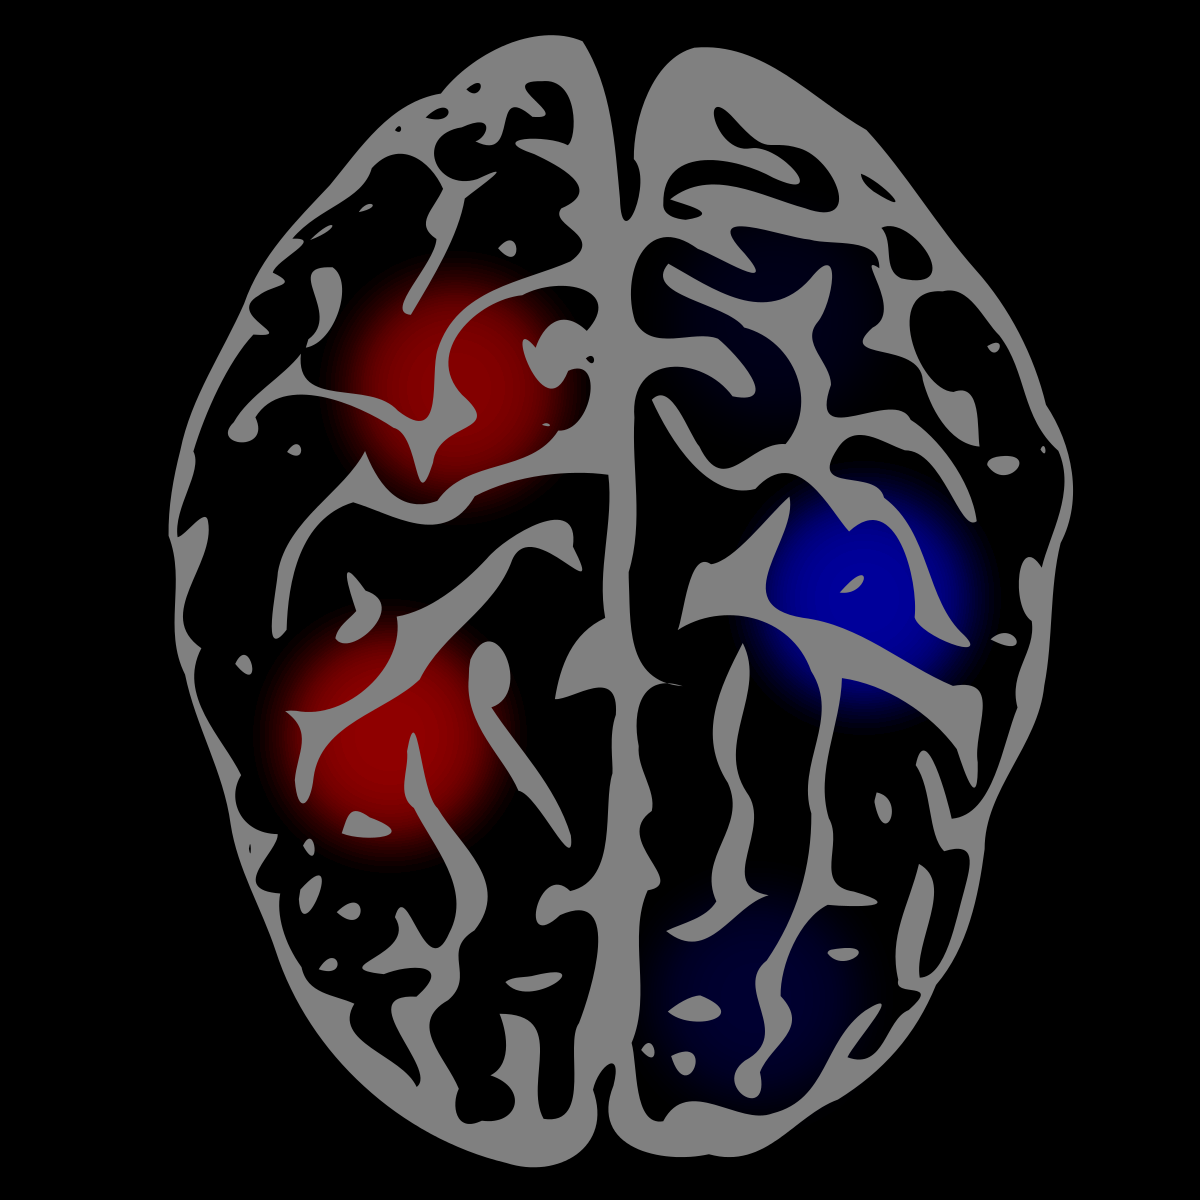
\includegraphics[scale = 0.10]{brain3.png} &
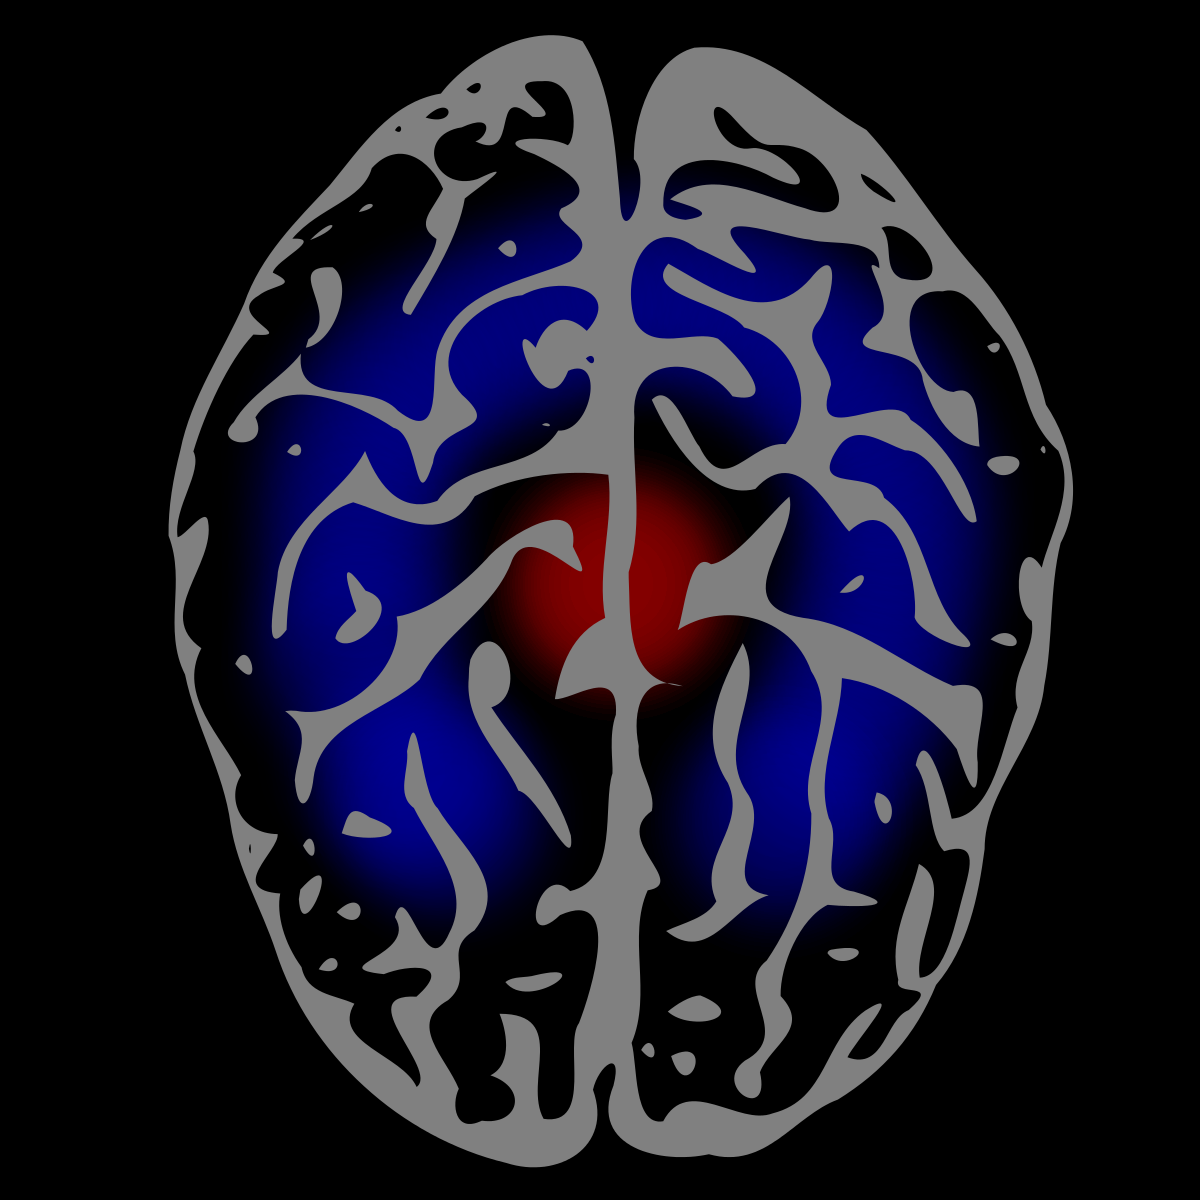
\includegraphics[scale = 0.10]{brain4.png} & $\cdots$\\ \hline
\end{tabular}
\end{center}
\end{block}




\begin{block}{Identification}
\begin{center}
\begin{tabular}{c|c|cccc}
\hline
$y^*$ &     & &  $i^* = ?$  &   \\
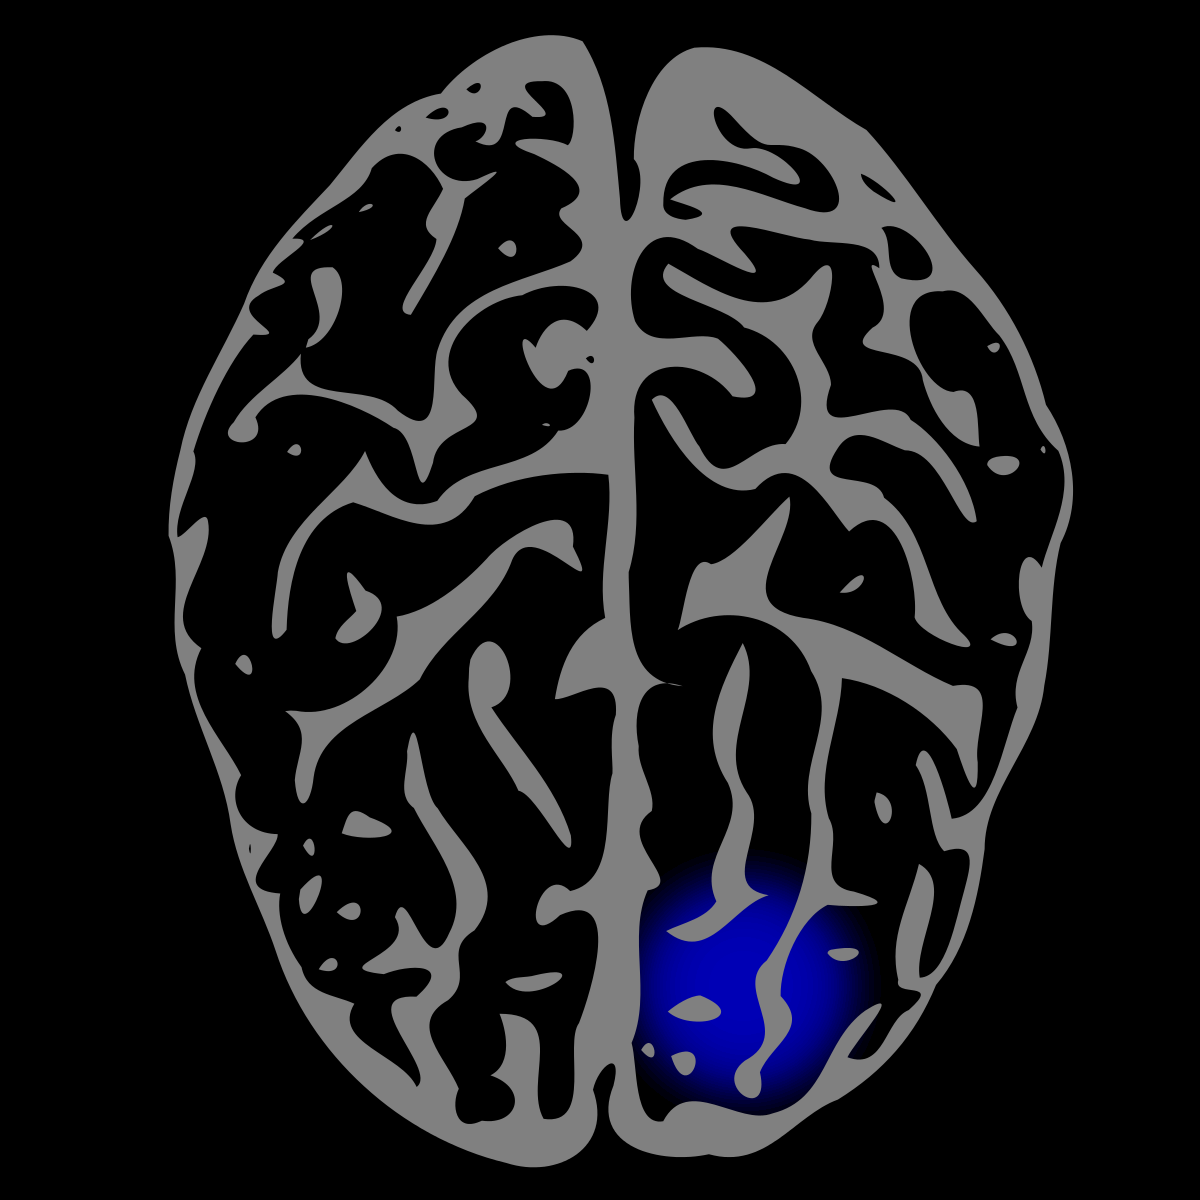
\includegraphics[scale = 0.09]{brain7.png} & \hspace{0.5in} 
& 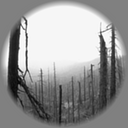
\includegraphics[scale = .7]{img5.png}
& 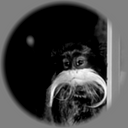
\includegraphics[scale = .7]{img6.png}
& 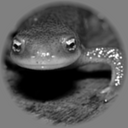
\includegraphics[scale = .7]{img7.png}
& 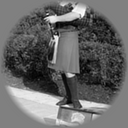
\includegraphics[scale = .7]{img8.png}\\
\hline
\end{tabular}
\end{center}
\begin{itemize}
\item Let $S$ be a set of stimuli, possibly outside the training set! $|S|$ can range from 120 to 10000
\item Scientist picks a stimulus $i^*$ from $S$ and measures the subject's reponse $y^*$
\item Can the statistician \emph{identify} $i^* \in S$ from $y^*$?
\item \emph{Objective}: minimize misclassification rate
\end{itemize}
\end{block}

\end{column} % End of the first column

\begin{column}{\sepwid}\end{column} % Empty spacer column



\begin{column}{\onecolwid}

%----------------------------------------------------------------------------------------
%	MATERIALS
%----------------------------------------------------------------------------------------



\begin{block}{Previous approaches}

\begin{itemize}
\item In order to generalize to new stimuli, we need to find some quantitative representation
\item Kay (2008) uses \emph{Gabor filters} to describe each picture in terms of $q = 10000$ real-valued features
\begin{center}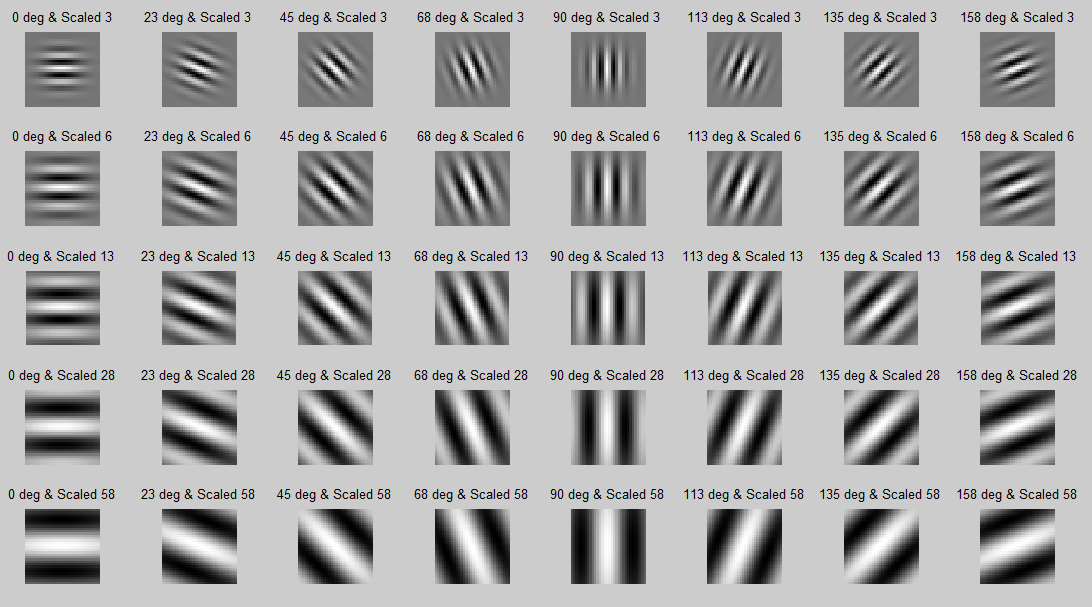
\includegraphics[scale = 0.7, trim = 0in 2.5in 0in 0in, clip]{gabor.png}
\end{center}
\item $Y_{T \times p}$ matrix containing the $T$ of recorded responses
\item $X_{T \times q}$ matrix of the \emph{image features} of the corresponding stimuli
\item Correct featurization is crucial... but outside the scope of the current work
\end{itemize}

Consider a parametric model
\[
Y \sim F_\theta(X)
\]
Such a \emph{forward model} gives the distribution of the
response conditional on the stimuli features.

The \emph{maximum likelihood} (ML) principle can be invoked to
identify the stimuli $i \in S$ ``most likely'' to have produced $y^*$.
Let $x_i : i \in S$ denote features of the test stimuli, and
identify $y^*$
\[
i^* = \text{argmax}_i \ell_\theta(y^*| x_i)
\]

\emph{Example.} We take the following as a representative approach, combining features of [1] and [2]:
\begin{itemize}
\item Assume the normal mutivariate linear model
\[Y \sim N( XB , \Sigma_E), \text{ where }B \in \mathbb{R}^{q \times p}\]
\item Estimate $B$ using elastic net [4]
\item Estimate $\Sigma_E$ using off-diagonal shrinkage of sample covariance matrix of residuals
\item The ML rule takes the form
\begin{equation}\label{mlrule}
i^* = \text{argmin}_{i} (x_i^T \hat{B} - y^*)^T \hat{\Sigma}_E^{-1} (x_i^T \hat{B} - y^*)
\end{equation}
\end{itemize}
\end{block}

\begin{block}{Initial Questions}
\begin{itemize}
\item Consider the Gaussian model for now...
\item Is ML (or MAP) optimal for identification?
\item Suppose not, then can we find other rules of the form \eqref{mlrule}, by estimating $\hat{B}$ or $\hat{\Sigma}_E$ differently, which are near optimal?
\end{itemize}
\end{block}


%\begin{center}
%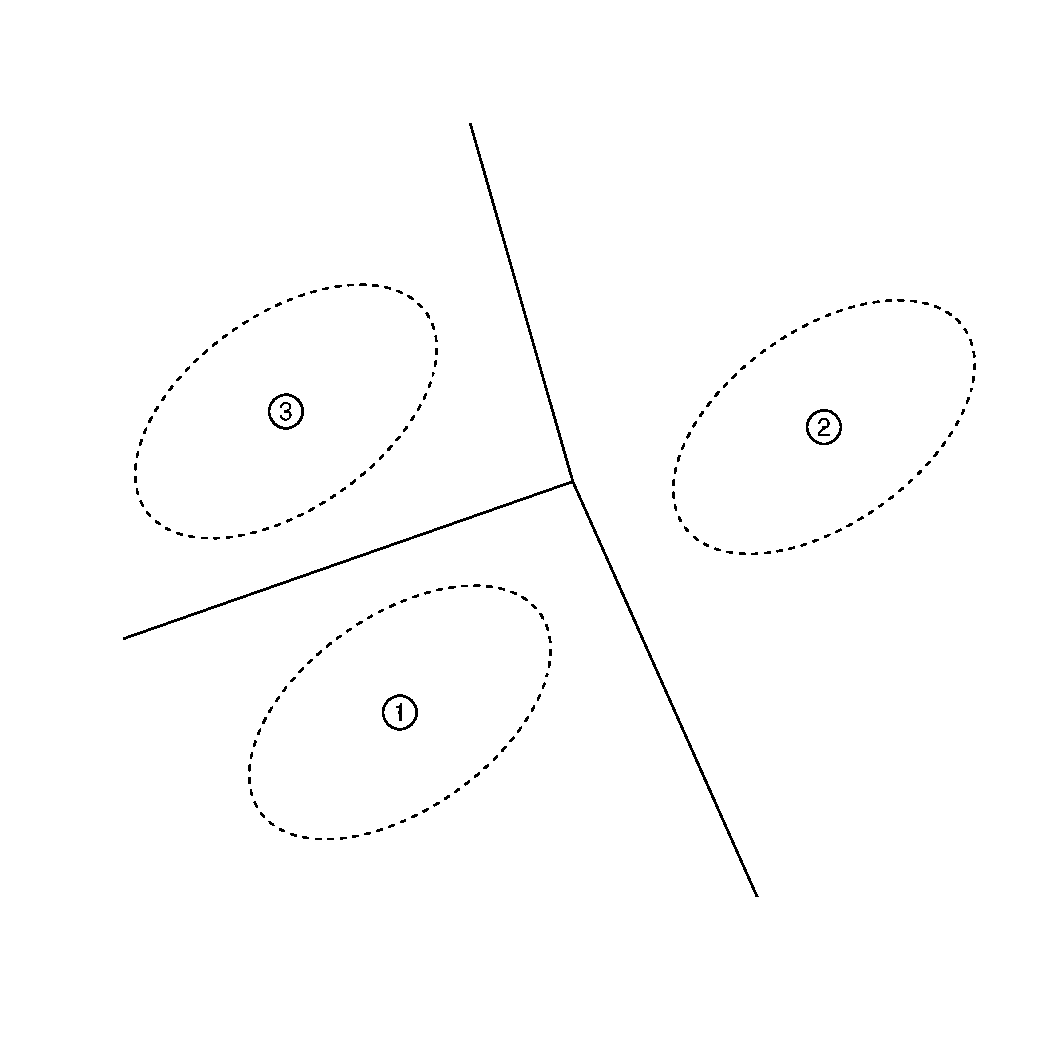
\includegraphics[scale = 1.0]{illus1_A.pdf}
%\end{center}

%\emph{Theoretical results}
%\begin{itemize}
%\item Asymptotic consistency to optimal procedure $T \to \infty$ under correct model specification
%\item Inconsistency given model misspecification (nonlinearity)
%\end{itemize}



%----------------------------------------------------------------------------------------

\end{column} % End of column 2.1

\begin{column}{\sepwid}\end{column} % Empty spacer column


\begin{column}{\onecolwid}

\begin{block}{Theory}
\begin{itemize}
\item ML is consistent given the correct model, but can be rather poor in finite samples
\item $\hat{B}$ minimizes squared error--but that isn't the loss function for identification!
\item We can compute optimal $\hat{B}$ for $p = q = 1$
\item Optimal rule of form \eqref{mlrule} intractable in higher dimensions due to nonconvexity
\end{itemize}
\begin{center}
\begin{tabular}{cc|c}
\multicolumn{2}{c}{\emph{Loss functions}} & {\emph{1D example}}\\
{\small Squared error} & {\small Identification} & {\small Optimal $\hat{B}$}\\
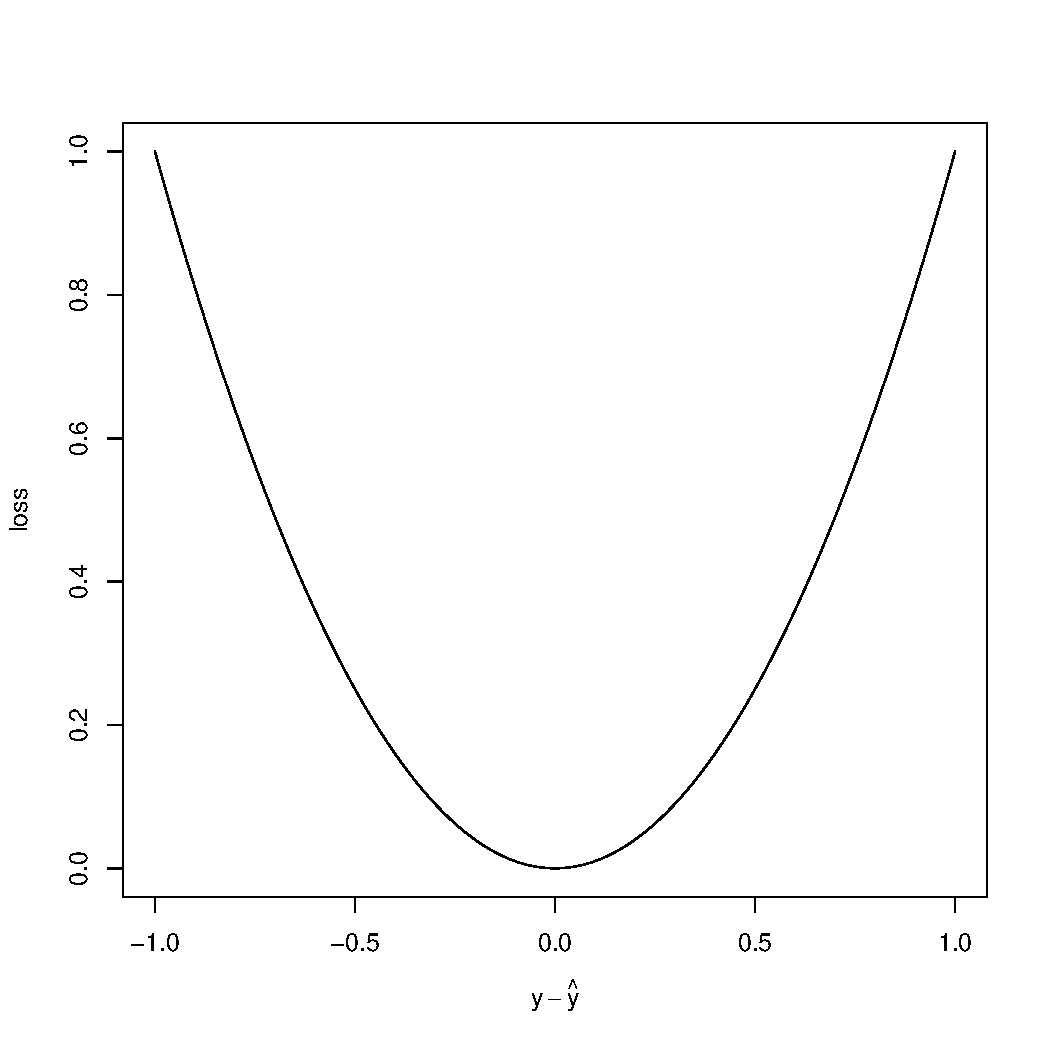
\includegraphics[scale = 0.6, trim = 1in 1in 0.5in 1in, clip]{loss_se.pdf} & 
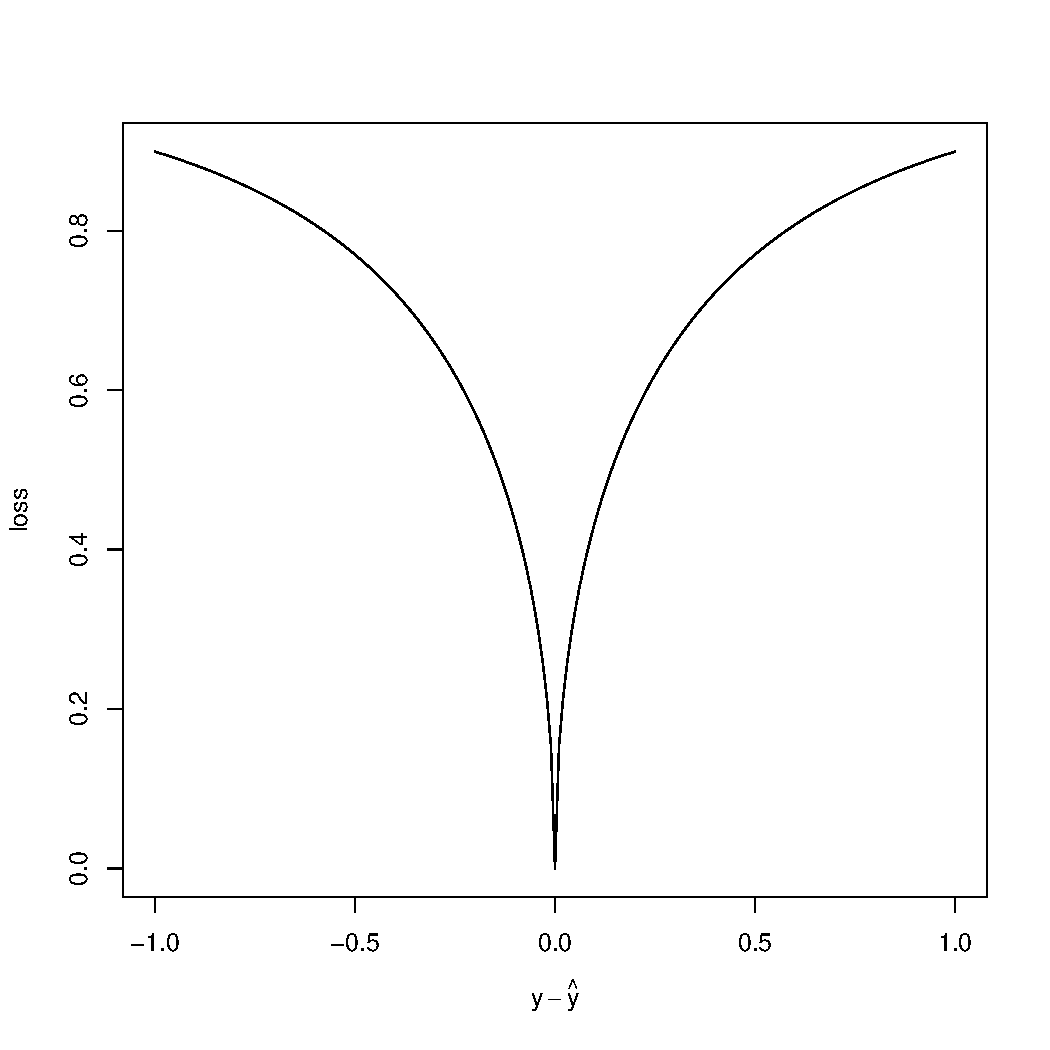
\includegraphics[scale = 0.6, trim = 1in 1in 0.5in 1in, clip]{loss_3.pdf} &
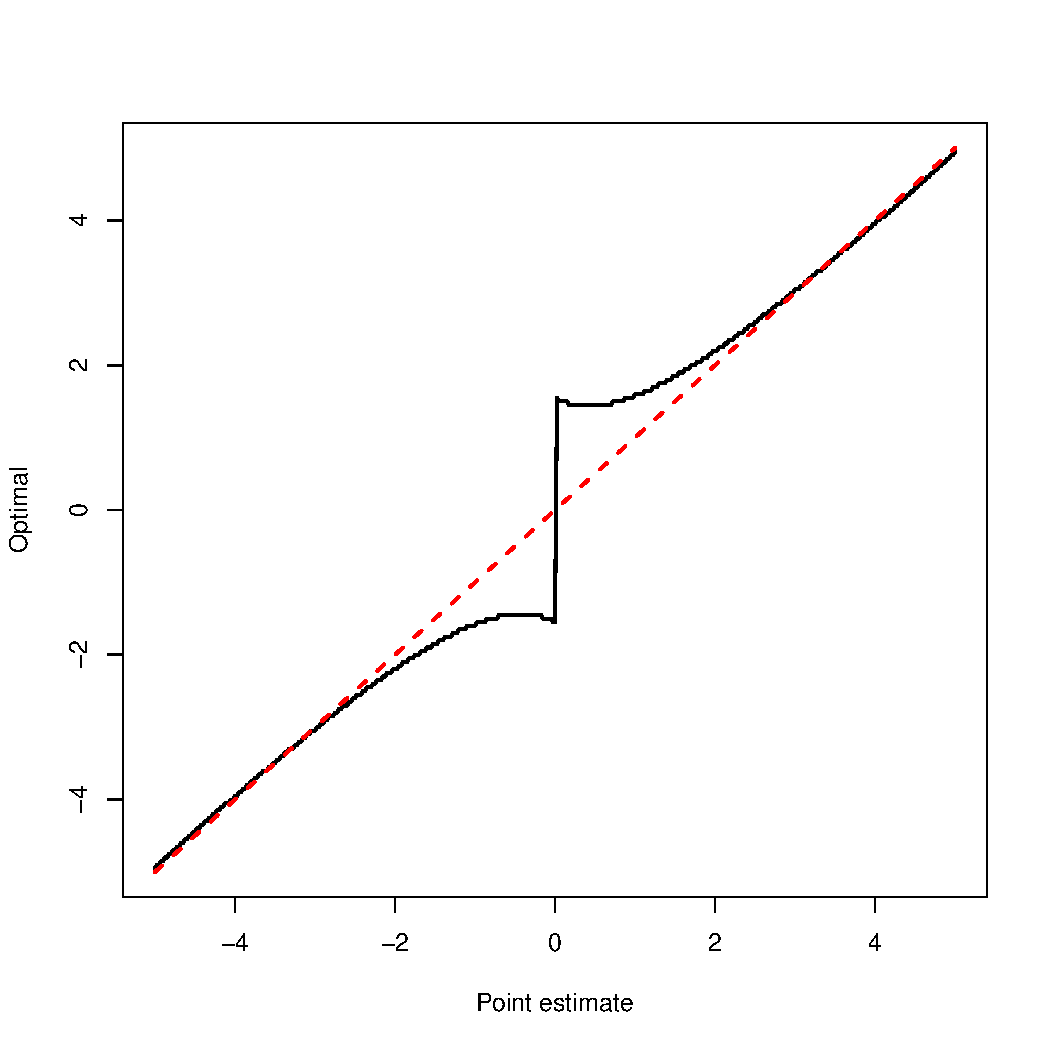
\includegraphics[scale = 0.6, trim = 1in 1in 0.5in 1in, clip]{zero2.pdf}\\
{\small 0} & {\small 0} & {\small 0}\\
{\small $ y - \hat{y}$} & {\small $y - \hat{y}$} & $\hat{B}_{ML}$
\end{tabular}
\end{center}
{\small
\emph{Right:} A $p = q = 1$-dimensional example where we can compare the optimal $\hat{B}$ to $\hat{B}_{ML}$.
They disagree around 0 since it is \emph{never} optimal to estimate $\hat{B}=0$ in identification (as opposed to regression, where $\hat{y} = 0$ is often a good estimate!)
}
\end{block}

\begin{block}{Empirical Bayes}

\begin{itemize}
\item \emph{Idea}: Unlike ML, the Bayes rule surely optimizes the ``correct'' objective function.  Can we approximate the Bayes rule?
\item \emph{Empirical Bayes}: use the data to estimate the covariances
$\Sigma_B$ and $\Sigma_E$, then compute posterior distribution of $B$
\item Assume coefficients of $B$ independent; diagonals of $\Sigma_B$ can be estimated using any estimate of signal strength, e.g. \emph{Eigenprism} [3].
\item Decision rule similiar to \eqref{mlrule} but with ``added noise'' due to uncertainty of $B$.
\[
\text{min} (x_i^T B - y^*)^T (\text{Cov}(x_i^T B) + \hat{\Sigma}_E)^{-1} (x_i^T B - y^*)
\]
\item Analogous to LDA vs QDA
\begin{center}
\begin{tabular}{cc}
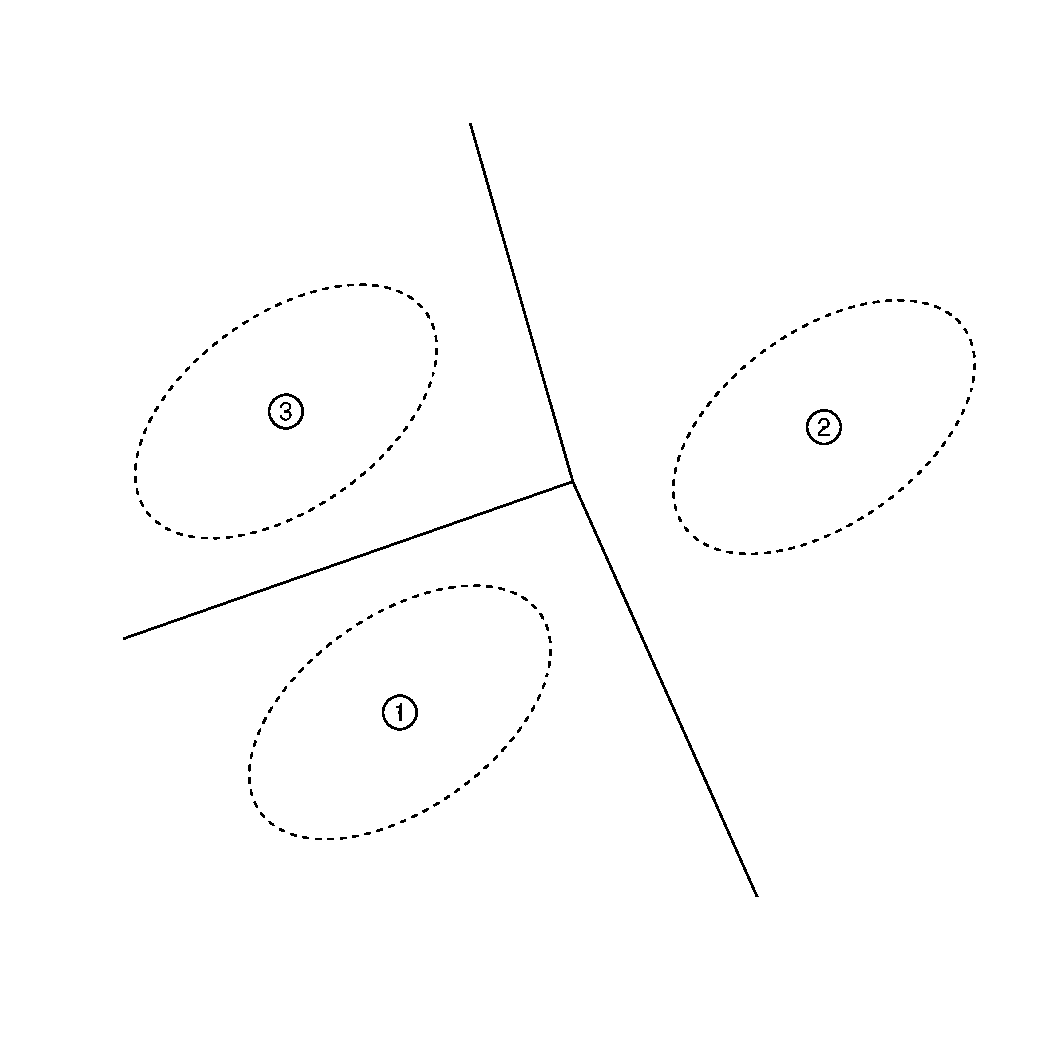
\includegraphics[scale = 0.5, trim = 0in 1.5in 0in 0in]{illus1_A.pdf} & 
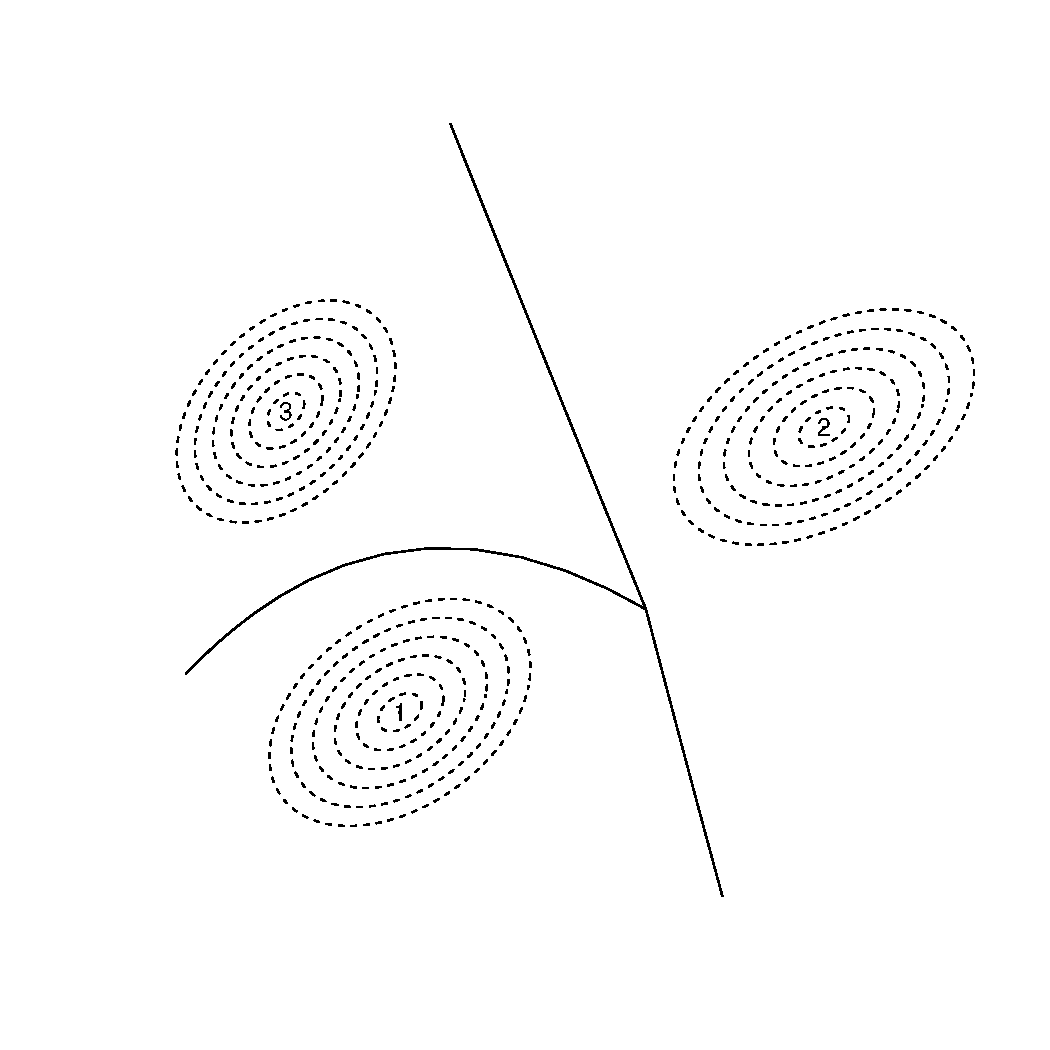
\includegraphics[scale = 0.5, trim = 0in 1.5in 0in 0in]{illus1_B.pdf}\\
ML & EB
\end{tabular}
\end{center}
\item \emph{Computation:} requires inverting $pq \times pq$ matrix
\end{itemize}

\end{block}





%----------------------------------------------------------------------------------------

\end{column} % End of column 2.2

\begin{column}{\sepwid}\end{column} % Empty spacer column

\begin{column}{\onecolwid} % The third column

%----------------------------------------------------------------------------------------
%	CONCLUSION
%----------------------------------------------------------------------------------------

\begin{block}{Simulation Results}
\begin{itemize}
\item Parameters $p = q = 60$, random $B$ and $\Sigma_E$, number of classes $|S| = 100$
\item Empirical bayes \emph{does} outperform ML given small sample sizes... however...
\end{itemize}
\begin{center}
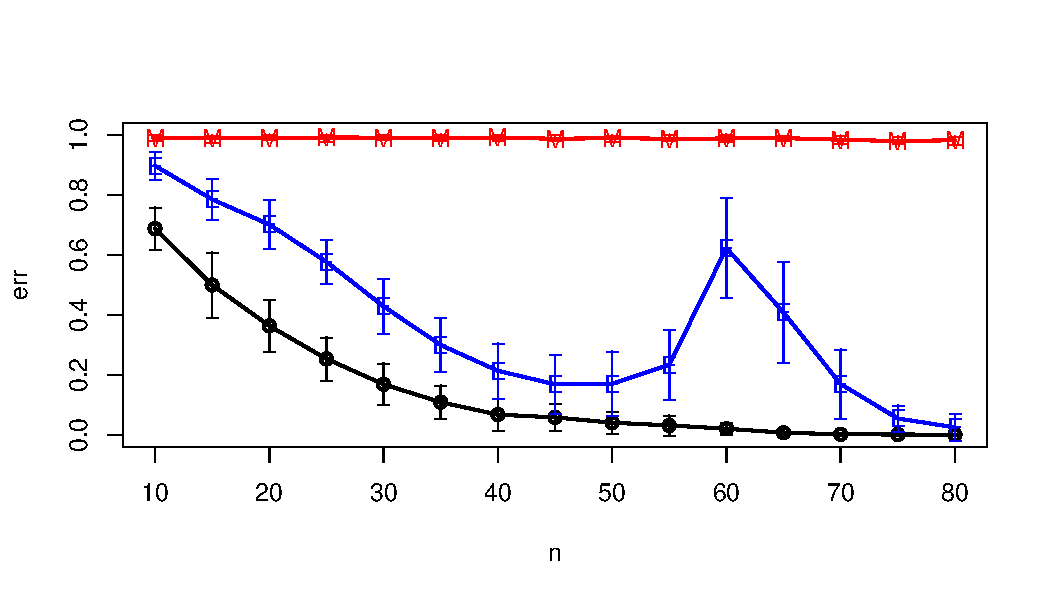
\includegraphics[scale = 1.3, trim = 0in 0in 0in 0.5in]{simulation1.pdf}
\end{center}
\small{
 \textcolor{blue}{(E)} Empirical Bayes,  \textcolor{red}{(M)} Maximum likelihood,
(o) Bayes risk \emph{(knowing true $\Sigma_B$, $\Sigma_E$)}}
\end{block}

\begin{block}{Ongoing Work}
\begin{itemize}
\item Why does error \emph{increase} with sample size!?
\item Clearly, we need to refine the EB procedure
\item Cost of $O((pq)^3)$ hinders application to real data... develop tractable approximations
\end{itemize}
\end{block}

\setbeamercolor{block alerted title}{fg=white,bg=Violet} % Change the alert block title colors
\setbeamercolor{block alerted body}{fg=black,bg=white} % Change the alert block body colors

\begin{block}{Conclusions}
\begin{itemize}
\item We studied optimal identification under the multivariate linear model
\item ``LDA''-like rules of the form \eqref{mlrule} (such as ML) are too restrictive.
But ``QDA''-like rules include the optimal Bayes rule!
\item We propose EB to approximate the Bayes rule-- but we need better theory to do it correctly
\end{itemize}
\end{block}

%----------------------------------------------------------------------------------------
%	REFERENCES
%----------------------------------------------------------------------------------------

\begin{block}{References}

\small{
\noindent [1] Kay et al. \emph{Nature} (2008)\\
\noindent [2] Vu et al. \emph{Annals of Applied Statistics} (2011)\\
\noindent [3] Janson et al. (2015) http://arxiv.org/abs/1505.02097\\
\noindent [4] Zou et al. \emph{J. R. Statist. Soc. B} (2005)
}

\end{block}

%----------------------------------------------------------------------------------------
%	ACKNOWLEDGEMENTS
%----------------------------------------------------------------------------------------

\begin{block}{Acknowledgements}


\small{ This work was supported by an NSF graduate research fellowship.
  We are also grateful to the travel support provided by the SAND 7 conference.  }

\end{block}




%----------------------------------------------------------------------------------------

\end{column} % End of the third column

\end{columns} % End of all the columns in the poster

\end{frame} % End of the enclosing frame

\end{document}
